% ============================================================
% Conteúdo acadêmico puro do documento "Diagrama de Implantação".
% SEM \documentclass, \begin{document}/\end{document} nem título —
% pensado para ser reaproveitado via \input{} tanto no documento
% modular quanto, futuramente, no TCC principal.
%
% Fonte do conteúdo: Diagrama_de_Implantacao.md e
% Implantacao_RadarTorres.puml (nesta mesma pasta), levantados a
% partir de installer/RadarTorres.iss, src/RadarTorres.App/App.xaml.cs,
% src/RadarTorres.App/RadarTorres.App.csproj e
% Docs/Tecnica/COMUNICACAO_ARDUINO.md.
% ============================================================

\section{Apresentação}

Este documento especifica o diagrama de implantação do sistema \textbf{RadarTorres}, descrevendo
a distribuição física dos componentes de software sobre os nós de hardware envolvidos: o
computador do usuário, onde roda a aplicação desktop, e o Arduino, responsável pela leitura dos
sensores e pelo acionamento das torres demonstrativas. Complementa o \emph{Diagrama de Classes}
(estrutura estática) e o \emph{Modelo de Banco de Dados} (persistência), mostrando onde cada
parte do sistema efetivamente executa e como os nós se comunicam.

O sistema representa apenas dois nós físicos reais --- computador do usuário e Arduino ---, sem
nenhum componente de servidor, web ou nuvem: trata-se de uma aplicação desktop única e
autocontida, comunicando-se com um único microcontrolador externo via porta serial.

\section{Nós e Elementos}

\begin{longtable}{p{4.6cm}p{4.2cm}p{6.0cm}}
  \caption{Nós e elementos do diagrama de implantação} \\
  \hline
  \textbf{Nó} & \textbf{Elemento} & \textbf{Papel} \\
  \hline
  \endfirsthead
  \multicolumn{3}{c}{\small \tablename~\thetable\ (continuação)} \\
  \hline
  \textbf{Nó} & \textbf{Elemento} & \textbf{Papel} \\
  \hline
  \endhead
  \hline
  \endfoot
  \small
  Computador do Usuário (Windows 10/11, 64-bit) & \texttt{RadarTorres.App} (.exe) & Único
  processo, self-contained (.NET 9), instalado por \texttt{installer/RadarTorres.iss}. \\
  \quad\llap{$\hookrightarrow$~}dentro do processo & Apresentação (\texttt{Views} +
  \texttt{ViewModels}) & Captura interação do operador, \emph{binding} declarativo
  (\texttt{ViewModelBase}, \texttt{RelayCommand}). \\
  \quad\llap{$\hookrightarrow$~}dentro do processo & Serviços (regra de negócio) &
  \texttt{ISerialCommunicationService}, \texttt{ITargetTrackingService},
  \texttt{ITowerSelectionService}, \texttt{IFireControlService}, \texttt{IZonaMortaService},
  \texttt{IAuthService}, \texttt{IPermissionService}. \\
  \quad\llap{$\hookrightarrow$~}dentro do processo & Persistência local & Leitura/escrita do
  banco SQLite via \texttt{Microsoft.Data.Sqlite} (\texttt{SqliteConnectionFactory} /
  \texttt{Sqlite*Repository}). \\
  \quad\llap{$\hookrightarrow$~}dentro do processo & .NET 9 Desktop Runtime & Embutido pelo
  instalador --- sem dependência externa a instalar. \\
  Arduino (microcontrolador) & Firmware & Lê sensores, envia leituras de alvo, recebe comandos e
  aciona as torres demonstrativas. \\
  Armazenamento local (disco do usuário) & \texttt{\%AppData\%\allowbreak\textbackslash
  RadarTorres\allowbreak\textbackslash Data\allowbreak\textbackslash radartorres.db} (SQLite) &
  Usuários, auditoria, objetos detectados, preferências e demais dados cadastrais; CSV permanece
  apenas como exportação manual da tela de Objetos Detectados. \\
  Sensores de detecção & --- & Ângulo + distância, alimentam o Arduino. \\
  Torres demonstrativas / indicador & --- & Laser de baixa potência ou LED, nunca armamento
  real. \\
\end{longtable}

\section{Diagrama de Implantação}

O diagrama representa apenas dois nós físicos reais: o computador do usuário e o Arduino,
conectados exclusivamente por USB/Serial. Fonte: \texttt{Implantacao\_RadarTorres.puml}
(PlantUML), nesta mesma pasta.

\begin{figure}[htbp]
  \centering
  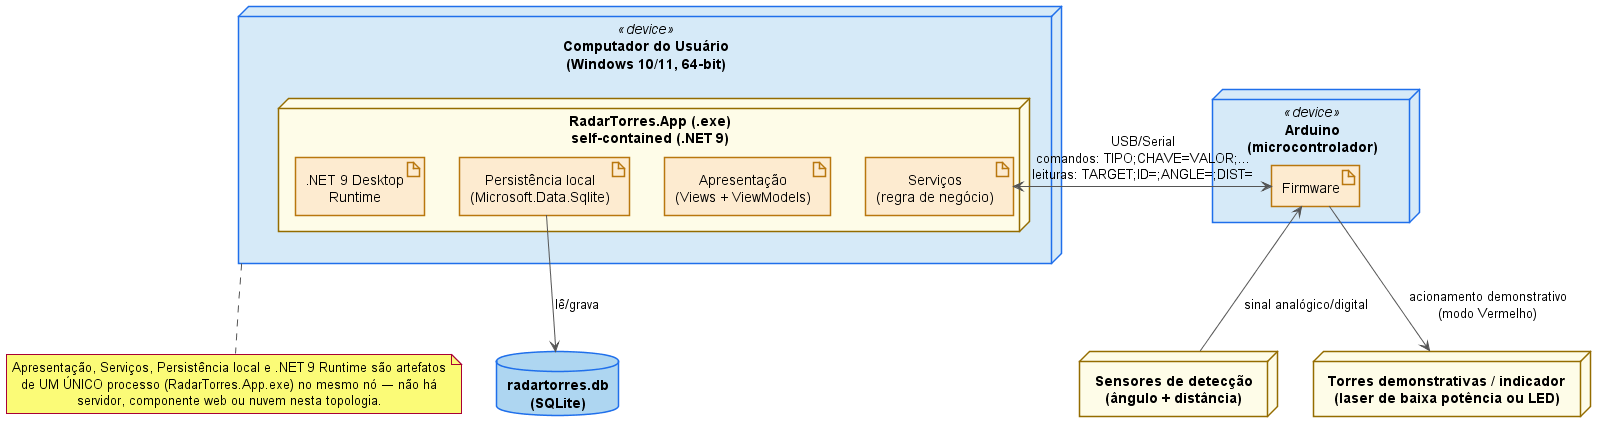
\includegraphics[width=\textwidth]{Implantacao_RadarTorres.png}
  \caption{Diagrama de implantação do RadarTorres.}
  \label{fig:implantacao}
\end{figure}

\section{Protocolo de Comunicação (USB/Serial)}

O único canal entre os dois nós físicos é a porta serial sobre USB, com mensagens em texto
simples (ver \texttt{Docs/Tecnica/COMUNICACAO\_ARDUINO.md} para a especificação completa) ---
Tabela~\ref{tab:protocolo}.

\begin{table}[htbp]
  \centering
  \caption{Mensagens trocadas no link serial}
  \label{tab:protocolo}
  \small
  \renewcommand{\arraystretch}{1.25}
  \begin{tabular}{p{3.2cm}p{4.6cm}p{5.2cm}}
    \hline
    \textbf{Direção} & \textbf{Formato} & \textbf{Finalidade} \\
    \hline
    Computador $\rightarrow$ Arduino & \texttt{TIPO;CHAVE=VALOR;...} & Comandos (troca de modo,
    acionamento, configuração) \\
    Arduino $\rightarrow$ Computador & \texttt{TARGET;ID=;ANGLE=;DIST=} & Leituras de alvo
    (ângulo + distância detectados) \\
    \hline
  \end{tabular}
\end{table}

Não há reconhecimento criptográfico nem autenticação no link serial --- a segurança do sistema
depende do controle de acesso físico ao cabo USB e do fato de o Arduino ser um periférico
dedicado, sem acesso a rede.

\section{Explicação}

O diagrama usa a notação UML padrão de implantação: \texttt{Computador do Usuário} e
\texttt{Arduino} são nós físicos marcados com o estereótipo \textbf{«device»}; dentro do nó do
computador, o processo \texttt{RadarTorres.App.exe} é um nó de ambiente de execução que contém
quatro \textbf{«artifact»} (Apresentação, Serviços, Persistência local, .NET 9 Runtime) ---
artefatos de software do mesmo processo, não componentes distribuídos em máquinas ou processos
separados. O banco de dados (\texttt{radartorres.db}) é representado com o ícone de cilindro
(\textbf{database}), reservado para dados persistidos pelo sistema. Os dois acoplamentos mais
relevantes do processo saem da caixa para fora: Serviços comunica-se com o Arduino pela porta
serial, e a camada de Persistência lê/grava o banco SQLite local em disco.

Do lado do Arduino, o Firmware concentra as quatro responsabilidades físicas do dispositivo: ler
os sensores de ângulo/distância, enviar leituras de alvo ao computador, receber comandos e
acionar as torres demonstrativas.

A escolha por um único processo desktop self-contained, sem servidor, é coerente com o argumento
de segurança/leveza já discutido para o SGBD (ver documento \emph{Modelo de Banco de Dados}):
menor superfície de ataque (nenhuma porta de rede exposta), zero administração de infraestrutura
e instalação totalmente local, adequadas ao perfil de nó único do protótipo.

\section{Conclusão}

O diagrama de implantação evidencia a natureza autocontida do RadarTorres: um único nó de
software (a aplicação desktop, self-contained sobre o .NET 9) comunicando-se com um único
microcontrolador externo via porta serial, sem qualquer dependência de infraestrutura de
servidor, web ou nuvem. Toda a persistência ocorre localmente, no próprio computador do usuário,
via SQLite, e a segregação em blocos internos (Apresentação/Serviços/Persistência/Runtime) é
apenas didática --- não representa componentes fisicamente distribuídos.

\section{Validação}

Nós, artefatos e protocolo confirmados em \texttt{installer/RadarTorres.iss},
\texttt{App.xaml.cs} e \texttt{Docs/Tecnica/COMUNICACAO\_ARDUINO.md}. Driver de persistência
(\texttt{Microsoft.Data.Sqlite} 9.0.0) confirmado em
\texttt{src/RadarTorres.App/RadarTorres.App.csproj:50}. A segregação em quatro blocos internos
(Apresentação/Serviços/Persistência/Runtime) é didática, não uma leitura de componentes
fisicamente distribuídos --- ver Seção 6 de \texttt{UML\_RadarTorres.md} (pasta \texttt{UML/}).
